\chapter{Approximate Matching of DNA Patterns}

Known as the central dogma (Figure \ref{fig:CentralDogma}, reprinted from Wikipedia), DNA makes RNA, and RNA directs the synthesis of proteins. Viral DNA indirectly produces viral proteins, which are probably drug targets. Identifying viral DNA patterns remains a challenge.

\begin{figure}
\centering
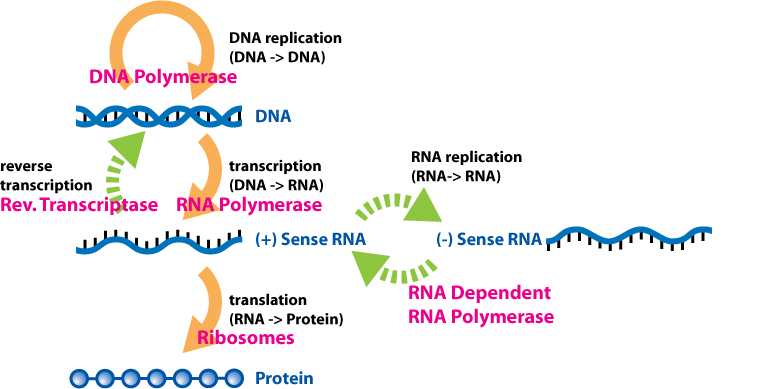
\includegraphics[width=\textwidth]{SequenceMatching/Figures/CentralDogma.jpg}
\caption{Central dogma of molecular biology. Figure reprinted from Wikipedia.}
\label{fig:CentralDogma}
\end{figure}

Recent decades have seen an explosion of emerging DNA data. The Human Genome Project \citep{681-1990,682-1998} revealed the complete human genome for the first time in 2003. The 1000 Genomes Project \citep{680-2008,679-2008} tries to discover the genomes of 1,000 human beings. Its scale is in the magnitude of 10\textsuperscript{12} base pairs.

The availability of such huge amounts of nucleotide sequences catalyzes the development of fast algorithms for approximate DNA string matching. Such algorithms should be able to tolerate errors due to mutations of nucleotides, which are adenine, cytosine, guanine, and thymine, or simply ACGT.

\section{Problem Definition}

Given a long text \textit{T} of alphabet ACGT, a short pattern \textit{P} of alphabet ACGTN where N is a wildcard, and an integer parameter \textit{K}, the problem is to find all the occurrences of subsequences from \textit{T}, such that their edit distances from \textit{P} are within \textit{K}. Edit distance is a similarity measure of two strings in terms of the number of primitive operations necessary to convert one string into an exact copy of the other. These primitive operations include substitution (e.g. AT\underline{T}T to AT\underline{G}T), insertion (e.g. AGT to A\underline{T}GT), and deletion (e.g. AT\underline{C}GT to ATGT). Transposition (e.g. AT\underline{TG} to AT\underline{GT}), however, is counted as two edit distances because it can only be achieved by at least two primitive operations. Usually the long text \textit{T} is the genome of a species, the pattern \textit{P} is the key pattern of interest, and the edit distance \textit{K} is the similarity control. Figure \ref{fig:ApproximateMatchingExample} shows an example of approximate DNA sequence matching.

\begin{figure}
\centering
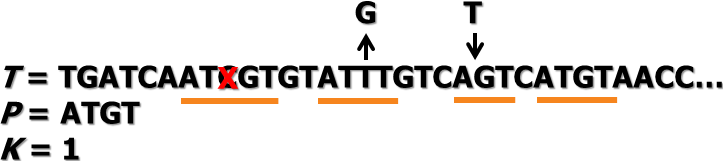
\includegraphics[width=\textwidth]{SequenceMatching/Figures/ApproximateMatchingExample.png}
\caption{Example of approximate DNA sequence matching.}
\label{fig:ApproximateMatchingExample}
\end{figure}

\section{Motivation}

This kind of problems has been studied intensively in the past two decades. New algorithms and programs for similar problems are continuously emerging. Approximate string matching algorithms can be categorized into online algorithms and offline algorithms. Online algorithms are used when the long text \textit{T} is unknown beforehand and thus cannot be preprocessed. In contrast, offline algorithms are used when the text is known in advance and thus can be preprocessed.

However, most existing online algorithms can only handle small scale problems. When querying large genomes, their performance becomes unacceptable. Offline algorithms such as Bowtie \citep{450-2009} and BWA \citep{251-2009} require building indexes, and their memory requirement is high.

Therefore, we were motivated by the desire to overcome the weakness of scalability of online algorithms. We developed a parallel implementation of  the traditional \textit{K}-difference agrep \citep{190-1992,451-1992} online algorithm for approximate nucleotide sequence matching by exploiting the huge computational power of modern NVIDIA GPU hardware using CUDA.

\section{Background}

For online algorithms, Wu and Manber \citep{190-1992,451-1992} developed agrep, which stands for approximate grep, as a traditional utility for online searching under Unix systems. Kiwi et al. \citep{703-2008} introduced a new dimension to online approximate string matching problem by introducing an error threshold parameter $\epsilon$ so that the algorithm is allowed to miss occurrences with probability $\epsilon$.

For offline algorithms, we \citep{197-2008} previously proposed an indexing structure called \textit{r}-cut numerical substring array (\textit{r}-NSA) to lower storage requirement. Kim et al. \citep{623-2007} proposed a new encoding method combining a suffix approach and a multi-pattern approach, claiming 5 times faster than agrep. Ghoting and Makarychev \citep{198-2009} proposed serial and parallel methods for I/O efficient suffix tree construction. Papamichail \citep{229-2009} presented a fast and linear space algorithm to calculate the edit distance of two strings. Srikantha et al. \citep{448-2010} made use of hash tables of \textit{Q}-grams, but the algorithm can only be used for exact-match searching, and the text \textit{T} is limited to 250 Mbp long. Aji et al. \citep{622-2010} ported the RMAP short-read mapping tool to GPU and resulted in impressive speedups of up to 14.5 times for the mapping kernel and up to 9.6-times for the overall program execution time. As for the state-of-the-art alignment tools, Bowtie \citep{450-2009} and BWA \citep{251-2009} aim to align a large amount of short reads to a reference genome in a fast manner by building sophisticated indexes based on Burrows-Wheeler transform.

Generally speaking, online algorithms can be applied in real time, hence they are particularly suitable for problems where the long text \textit{T} is either unknown in advance or changes frequently. Meanwhile, since they lack indexing structures, they require a longer execution time when compared to offline algorithms in case that the long text \textit{T} is reused for dozens of times, like aligning millions of short reads to a reference genome.

Our CUDA implementation builds no index at all, yet resulting in remarkably reduced execution time down to the scale of milliseconds. Meanwhile we also developed a multithreaded CPU counterpart using OpenMP for both validation and comparison. We name both programs CUDAagrep and OpenMPagrep respectively.

\section{Method}

\subsection{Binary Representation}

Nucleotides are either A, C, G or T. Since the alphabet size is 4, each nucleotide can be represented by only 2 bits. In this way, up to 4 nucleotides can be packed in a single byte. Similarly, up to 16 nucleotides can reside in a 32-bit integer. When genomes are loaded from disk into memory, all the nucleotides are converted into their binary representations. Therefore, the memory requirement of human genome, whose size is 3.10 Gbp, is merely 738 MB, exactly one fourth of its genome size.

\subsection{Agrep Algorithm}

The traditional \textit{K}-difference agrep algorithm maintains \textit{K}+1 matching tables, where \textit{K} is the edit distance with substitution, insertion, and deletion having a uniform cost of one. In the first iteration, their first columns are initialized. Then in subsequent iterations, a new column is calculated by logically or-ing four vectors, which respectively account for matching, substitution, deletion, and insertion, and then by appending an additional 1 to the end of the newly computed vector. An approximate matching is found when the last row is one. Since the pattern \textit{P} is stored in a machine word, logical operations guarantees bit parallelism. Because of this, however, the maximum pattern length is limited to 64. Readers are advised to refer to the original paper \citep{190-1992,451-1992} for programming detail.

The traditional agrep algorithm uses 1 to specify an approximate matching. In contrast, our implementation uses 0 instead in order to save the effort of appending an additional 1 when shifting vectors during iterations. Hence an approximate matching within \textit{K} edit distances is found when the last row of the last matching table equals 0. According to our in-house experiment, a performance improvement by 8\% was observed.

Figure \ref{fig:AgrepMatchingTables} shows an example of agrep matching tables denoted by R. In this example, the text \textit{T} is ACACATT, the pattern \textit{P} is ATT, and the edit distance \textit{K} is equal to 1. Hence there are two matching tables, namely R$_0$ and R$_1$. The red circle in R$_0$ indicates an exact matching, while the two red circles in R$_1$ indicate two approximate matchings, allowing 1 error.

\begin{figure}
\centering
\begin{tabular} {cc}
 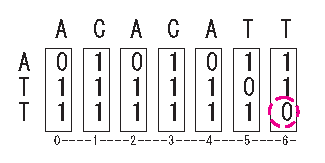
\includegraphics[width=0.45\textwidth]{SequenceMatching/Figures/AgrepMatchingTableR0.eps} &
 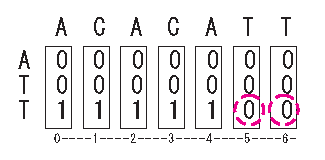
\includegraphics[width=0.45\textwidth]{SequenceMatching/Figures/AgrepMatchingTableR1.eps}\\
 R$_0$ & R$_1$ \\
\end{tabular}
\caption{Example of agrep matching tables.}
\label{fig:AgrepMatchingTables}
\end{figure}

\subsection{CUDA Implementation}

The performance of a CUDA program vastly depends on appropriate utilization of various memory spaces of a CUDA device (Figure \ref{fig:CUDAMemorySpaces}, reprinted from CUDA C Best Practices Guide v4.0, NVIDIA), which have different characteristics that reflect their distinct usages. Global memory has a large capacity, e.g. 1 GB on a modern graphics card, but have the greatest latency. Constant memory is cached and read-only, enabling fast access of globally constant values. Shared memory is on-chip and can be read and written by threads in a block for them to communicate and exchange data. Registers are very fast but scarce resources, so they should be used to store the most frequently updated variables.

\begin{figure}[t]
\centering
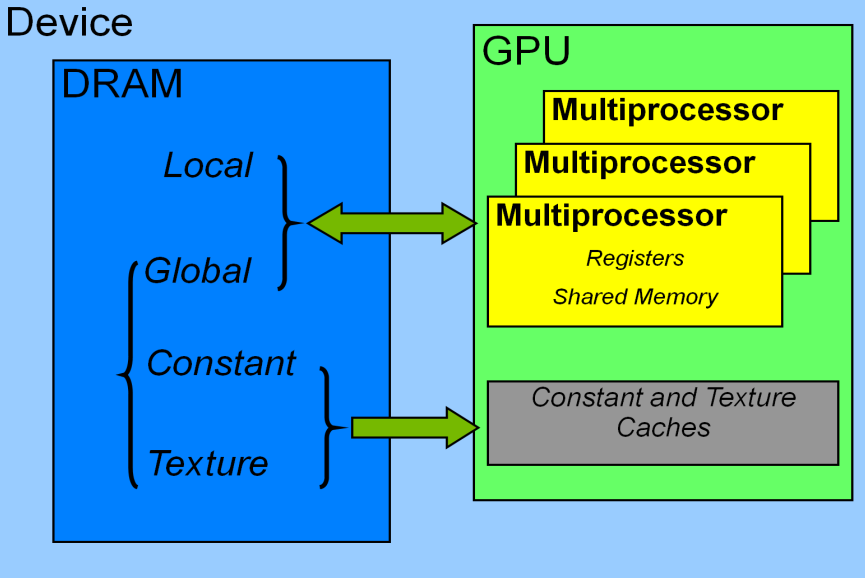
\includegraphics[width=\textwidth]{SequenceMatching/Figures/CUDAMemorySpaces.png}
\caption{Memory spaces of a CUDA device. Figure reprinted from CUDA C Best Practices Guide v4.0, NVIDIA.}
\label{fig:CUDAMemorySpaces}
\end{figure}

CUDAagrep is a CUDA implementation of agrep algorithm. Figure \ref{fig:CUDAagrepFlowchart} shows its overall flowchart. CUDAagrep costs about 40s to load the given genome from disk into main memory, and less than 1s to transfer the genome from main memory to GPU global memory. Inside a loop during searching, CUDAagrep transfers one pattern to GPU constant memory, invokes the agrep kernel, transfers the positions of matchings back to main memory, and dumps them to disk. It then processes the next pattern in an identical manner until all are done.

\begin{figure}
\centering
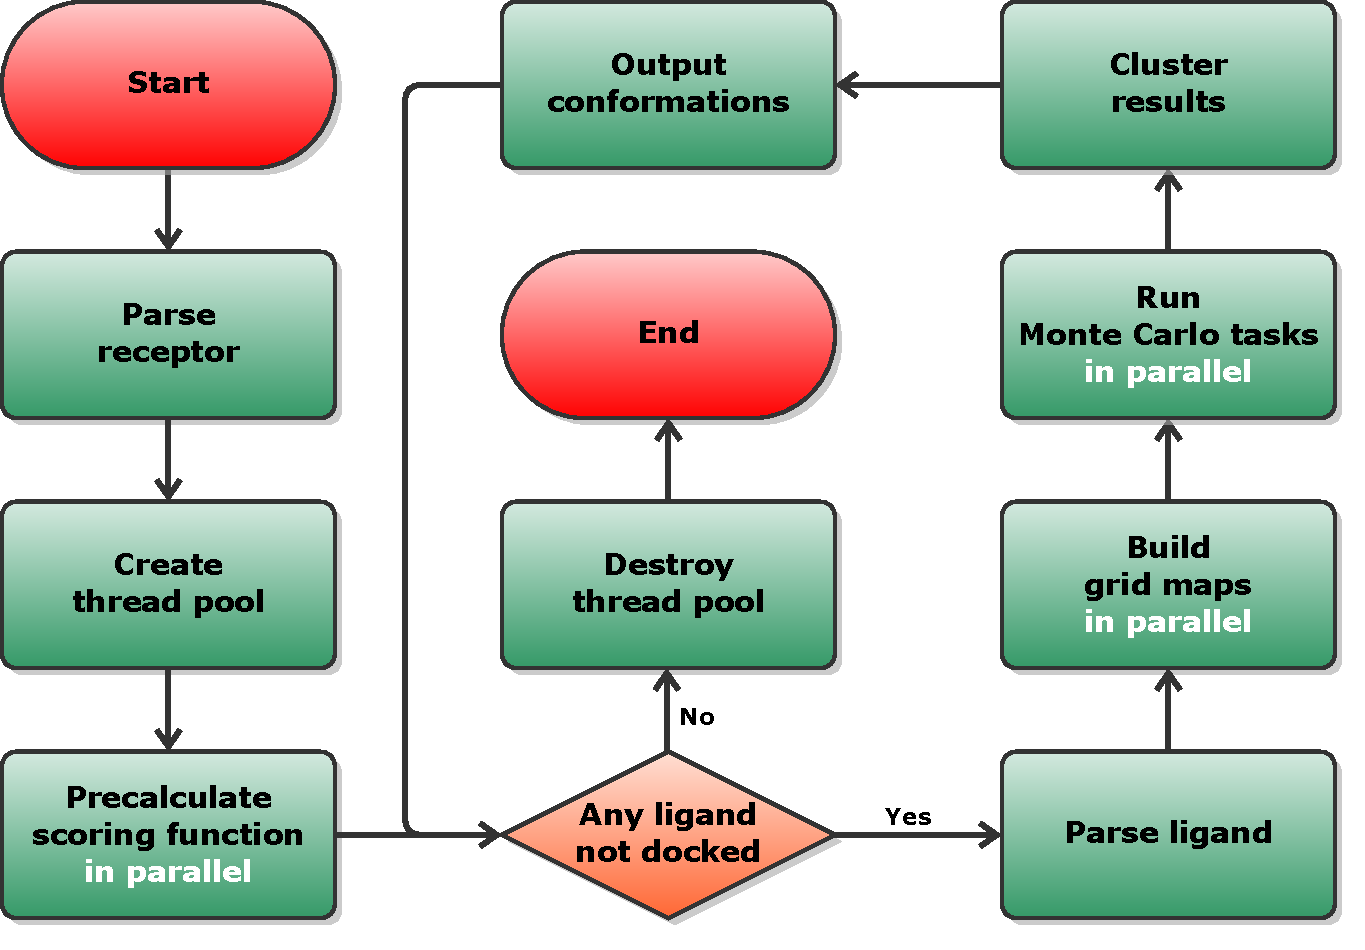
\includegraphics[width=\textwidth]{SequenceMatching/Figures/Flowchart.pdf}
\caption{Flowchart of CUDAagrep.}
\label{fig:CUDAagrepFlowchart}
\end{figure}

CUDAagrep boosts the searching step by exploiting subgenome level parallelism. The entire genome is first equally divided into multiple subgenomes, which are then distributed across a 1D domain of lightweight CUDA threads. In the current implementation, each CUDA thread processes 256 integers, i.e. 4,096 nucleotides. In a straightforward manner, the first thread processes the first 256 integers, the second thread processes the second 256 integers, and the like. This naive approach is functionally correct but unfortunately suffers from a performance issue when running on GPU. At a time, from GPU global memory, thread 0 fetches integer 0, thread 1 fetches integer 256, and thread 2 fetches integer 512, and so on. These integers are separated and far away from each other. Multiple memory transactions are required to fetch them all, which turn out to be a sharp performance drop. To tackle this issue in CUDAagrep, the integers are deliberately shuffled so that integers 0, 256, 512 and so on are adjacent to one another and reside in a region where only one memory transaction is needed. Likewise, integers 1, 257, 513 and so on are also shuffled. Figure \ref{fig:GenomeShuffling} demonstrates our idea in shuffling the integers in order to satisfy the requirements of global memory coalesced access. The numbers in cells are the indexes of integers in the original sequence.

\begin{figure}[t]
\centering
\subfigure[High-level layout.]
{
  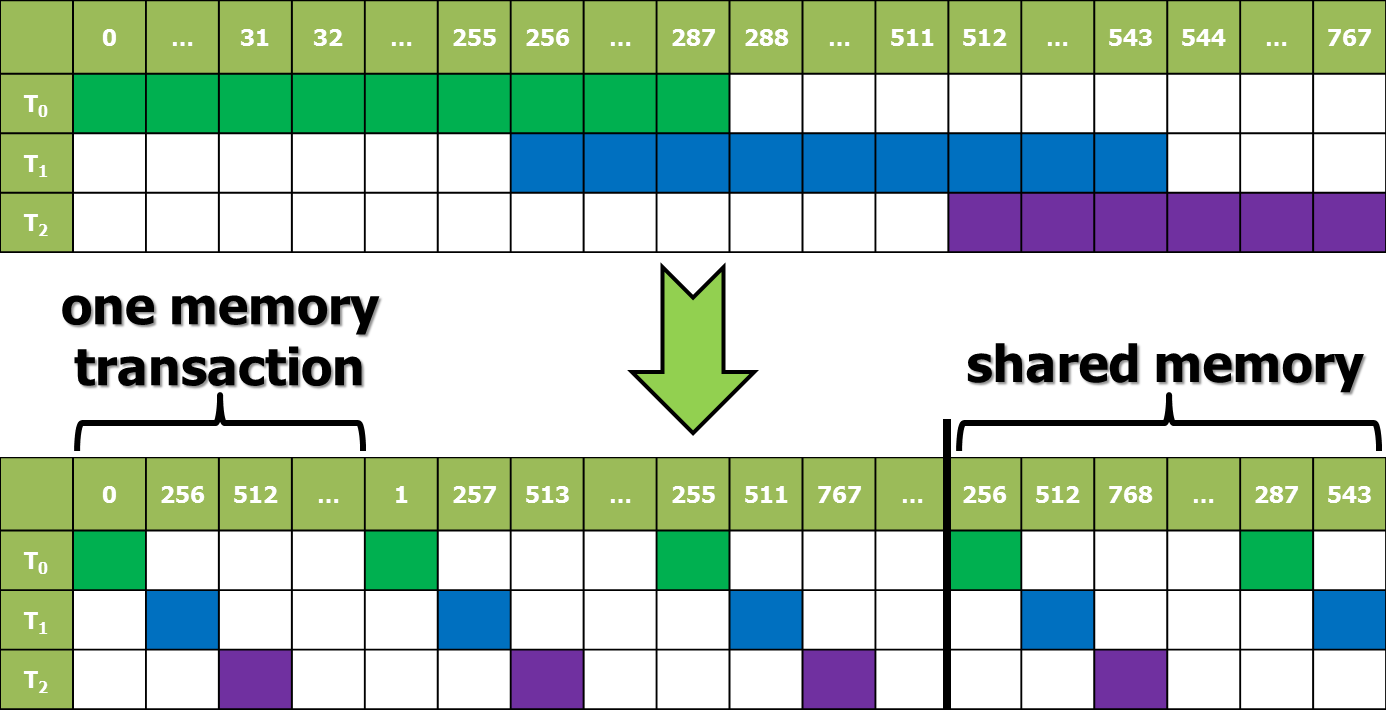
\includegraphics[width=\textwidth]{SequenceMatching/Figures/HighLevelLayoutGenomeShuffling.png}
  \label{subfig:HighLevelLayoutGenomeShuffling}
}
\subfigure[Low-level layout.]
{
  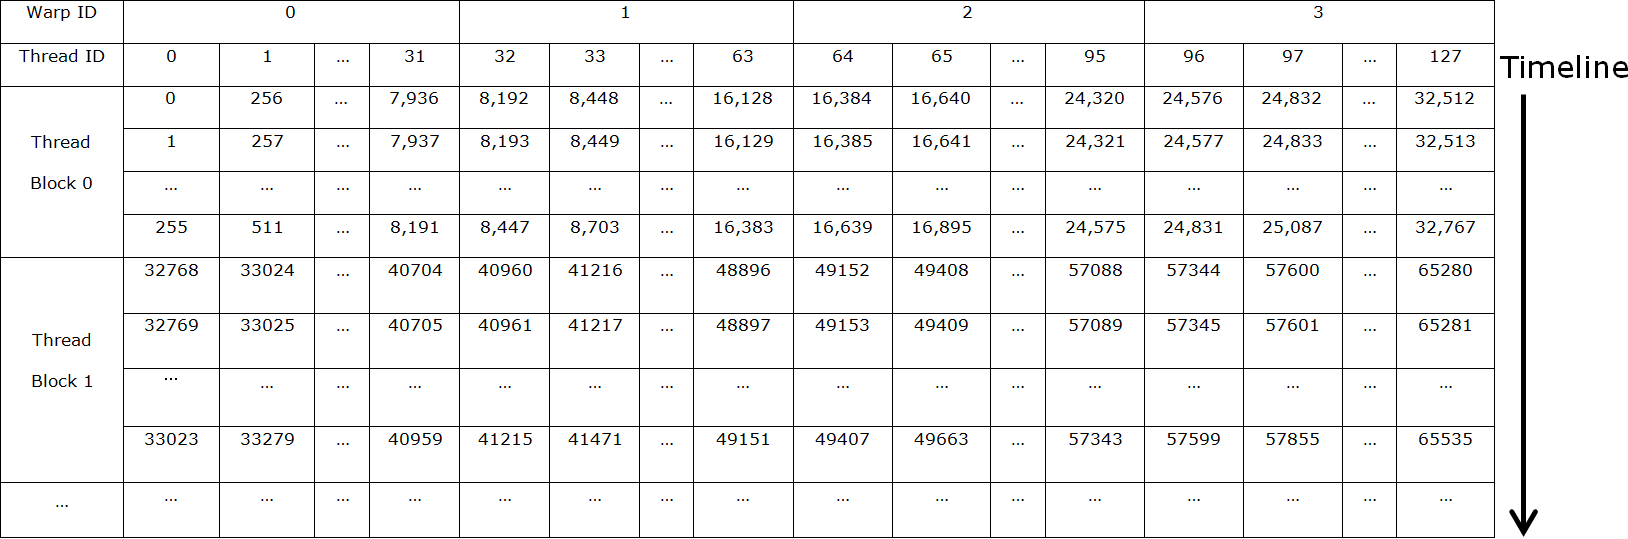
\includegraphics[width=\textwidth]{SequenceMatching/Figures/LowLevelLayoutGenomeShuffling.png}
  \label{subfig:1LI4-ZINC19888543}
}
\caption{Layouts for genome shuffling to satisfy coalesced access.}
\label{fig:GenomeShuffling}
\end{figure}

CUDAagrep guarantees no potential matchings are missing by allocating 32 additional integers to each thread for initializing the matching tables. Hence there are overlapping integers between two adjacent threads. CUDAagrep stores these overlapping integers into GPU shared memory, saving the effort of reloading them from global memory.

CUDAagrep fully utilizes on-chip GPU registers to directly save the matching tables which are frequently updated from iteration to iteration. In CUDAagrep, registers are organized in the form of indexable array at compile time. Since the number of matching tables is equal to \textit{K + 1}, where \textit{K} is the edit distance, multiple agrep kernels have to be defined, each with a fixed \textit{K} value.

CUDAagrep caches constant values and kernel arguments by saving them into GPU constant memory, enabling fast fetching.

\section{Experiments and Results}

CUDAagrep and OpenMPagrep were tested for searching for subsequences from 17 large genomes of different species whose sizes vary from 0.19 Gbp to 3.50 Gbp. Both programs were run on the same PC Xeon W3520 (2666 MHz), 8GB DDR3-1333 SDRAM, and GeForce GTX 285 (1024 MB) under Windows 7 x64. The QuadCore CPU supports Intel's Hyper-Threading technology and is thus able to execute up to eight threads simultaneously.

Figure \ref{fig:CUDAagrepQueryingTime} plots the average CUDAagrep querying times of 3 patterns, which were retrieved from the 17 genomes plus a few random amendments, against the genome sizes with edit distances of 0, 3, 6 and 9. The result concludes that for a fixed genome size, the average querying time increases linearly as edit distance, and for a fixed edit distance, it increases linearly as genome size.

\begin{figure}
\centering
\subfigure[Searching 17 genomes for patterns of length 30 with edit distances from 0 to 9.]
{
  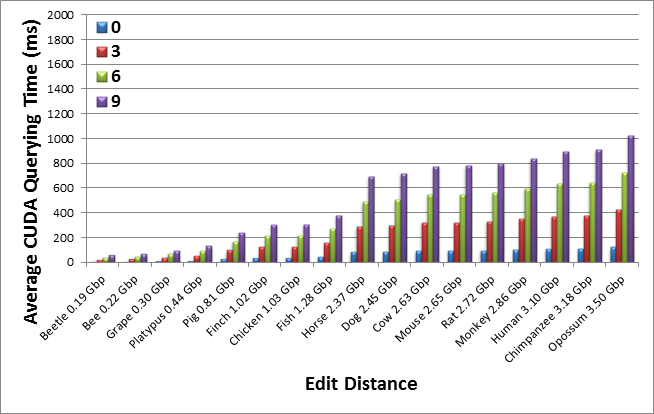
\includegraphics[width=\textwidth]{SequenceMatching/Figures/AverageCUDAagrepQueryingTimeM30.png}
}
\subfigure[Searching 17 genomes for patterns of length 60 with edit distances from 0 to 9.]
{
  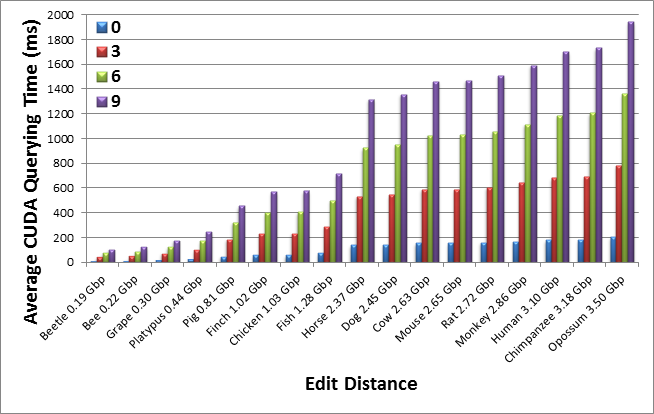
\includegraphics[width=\textwidth]{SequenceMatching/Figures/AverageCUDAagrepQueryingTimeM60.png}
}
\caption{CUDAagrep querying times against edit distances.}
\label{fig:CUDAagrepQueryingTime}
\end{figure}

Figure \ref{fig:PerformanceComparison} plots the average CUDAagrep and OpenMPagrep querying times of 3 patterns, which were retrieved from human genome plus a few random amendments, against the edit distances from 0 to 9. When the pattern length is 30 and the edit distance is 3, the OpenMP program requires about 26 seconds to complete one query on average, while the CUDA program merely costs 371 milliseconds, achieving a 70-fold speedup. When the pattern length is increased to 60 and the edit distance is increased to 6, the average querying time required by the CUDA program is only 1,188 milliseconds, achieving a 36-fold speedup compared to about 42 seconds required by the OpenMP program. The speedup drops to a half because CUDA consumes two 32-bit registers to emulate one 64-bit register internally to save the mask array of pattern of length 60.

\begin{figure}
\centering
\subfigure[Searching human genome for patterns of length 30 with edit distances from 0 to 9.]
{
  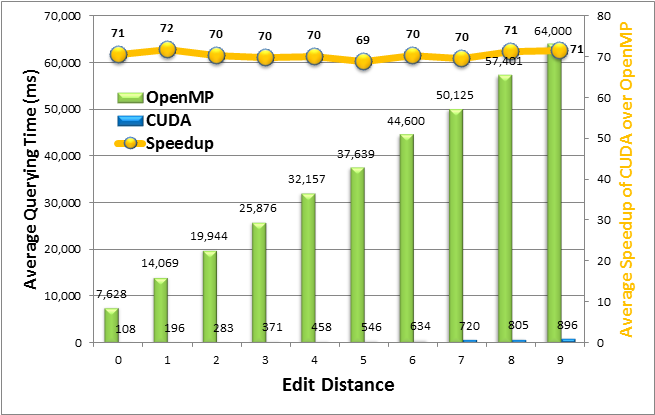
\includegraphics[width=\textwidth]{SequenceMatching/Figures/PerformanceComparisonHumanM30.png}
}
\subfigure[Searching human genome for patterns of length 60 with edit distances from 0 to 9.]
{
  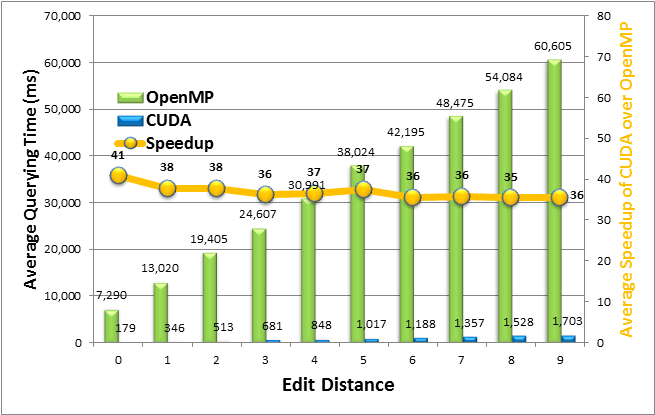
\includegraphics[width=\textwidth]{SequenceMatching/Figures/PerformanceComparisonHumanM60.png}
}
\caption{Performance comparison between CUDAagrep and OpenMPagrep against edit distances.}
\label{fig:PerformanceComparison}
\end{figure}

It can also be concluded that the speedup depends on the pattern length but not on the edit distance. It is natural to ask if the speedup also depends on the genome size. Therefore we tested both programs by searching 17 genomes of different sizes for patterns of lengths 20, 30, 40, 50 and 60, and plotted figure \ref{fig:SpeedupAgainstGenomes}, from which no correlation between the two can be found. Interesting enough, the three curves whose lengths exceed 32 perfectly overlap with each other.

\begin{figure}
\centering
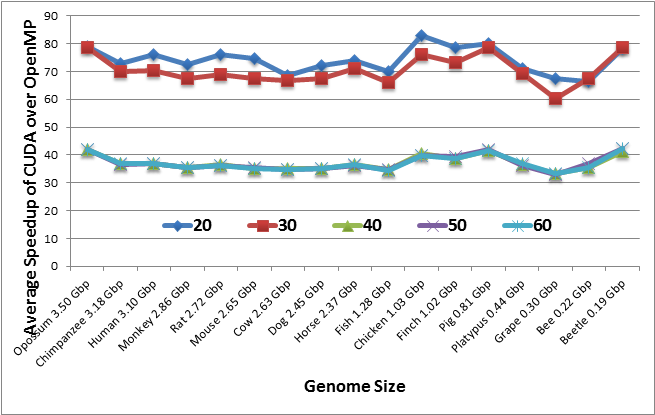
\includegraphics[width=\textwidth]{SequenceMatching/Figures/SpeedupAgainstGenomes.png}
\caption{Speedups of CUDAagrep over OpenMPagrep against genomes.}
\label{fig:SpeedupAgainstGenomes}
\end{figure}

\section{Discussion}

CUDAagrep complements, but not competes with, state-of-the-art alignment tools such as Bowtie \citep{450-2009} and BWA \citep{251-2009}, which aim to align a large amount of short reads to a reference genome. The underlying problems they try to solve are somewhat different. CUDAagrep enables biologists to conveniently search a genome of interest for a small amount of patterns with edit distance as the similarity measurement, and instantly get to know the number of matchings and their positions for each pattern, either by executing the program, browsing our website, or sending emails.

It is generally unfair to compare an online approach without index to an offline approach with indexes. Lacking an index, CUDAagrep cannot run as fast as Bowtie or BWA. However, CUDAagrep does not require building indexes of any kind, so new genomes can be downloaded and searched instantly. Therefore, CUDAagrep is especially suitable for scenarios where the long text \textit{T} is unknown beforehand or changes frequently.

Another advantage of CUDAagrep is its high sensitivity, which measures the proportion of actual positives which are correctly identified. It is calculated as the ratio of number of mapped reads over number of total reads. Since the reference genome is scanned through for each query without using any heuristic means, CUDAagrep is guaranteed not to miss any possible approximate matchings. The Escherichia coli sample data accompanied with the Bowtie package is used as test data. The e\_coli\_1000.fa file contains a set of 1,000 35-bp reads simulated from E. coli genome. Under single-end mode, 437, 349 and 341 out of 1,000 reads have at least one reported alignment respectively for CUDAagrep, Bowtie and BWA, resulting in sensitivities of 43.7\%, 34.9\% and 34.1\%. Under paired-end mode, 830, 706 and 703 out of 1,000 reads have at least one reported alignment respectively for CUDAagrep, Bowtie and BWA, resulting in sensitivities of 83.0\%, 70.6\% and 70.3\%. In other words, CUDAagrep achieves a 25.2\% higher sensitivity under single-end mode and a 17.6\% higher sensitivity under paired-end mode.

\section{Availability}

We have provided both x86 and x64 executables of CUDAagrep for both Linux and Windows at http://agrep.cse.cuhk.edu.hk. The C++ source code is licensed under Apache License 2.0, so users are encouraged to modify and recompile the source code to suit their own needs. API documentations are also available at our website. Since CUDAagrep requires no index, the reference genomes can be distributed over Internet in any format. Compressed formats are preferred in order to save network bandwidth. 7zip is well known for its high compression ratio, so the 17 7-zipped genomes are available for download from our website.

In addition, our website provides online real time searching by employing fruitful AJAX and MVC technologies including animations as well as asynchronous communications, aiming to supply users with rich experiences (Figure \ref{fig:CUDAagrepWeb}). Furthermore, we have also developed an email crawler to receive jobs via emails. Users can send emails to CUDAagrep@Gmail to queue up for a job (Figure \ref{fig:CUDAagrepEmail}). In both ways, hardware and software installation and configuration are not needed at all, so potential users can benefit from our tool to a maximum extent.

\begin{figure}
\centering
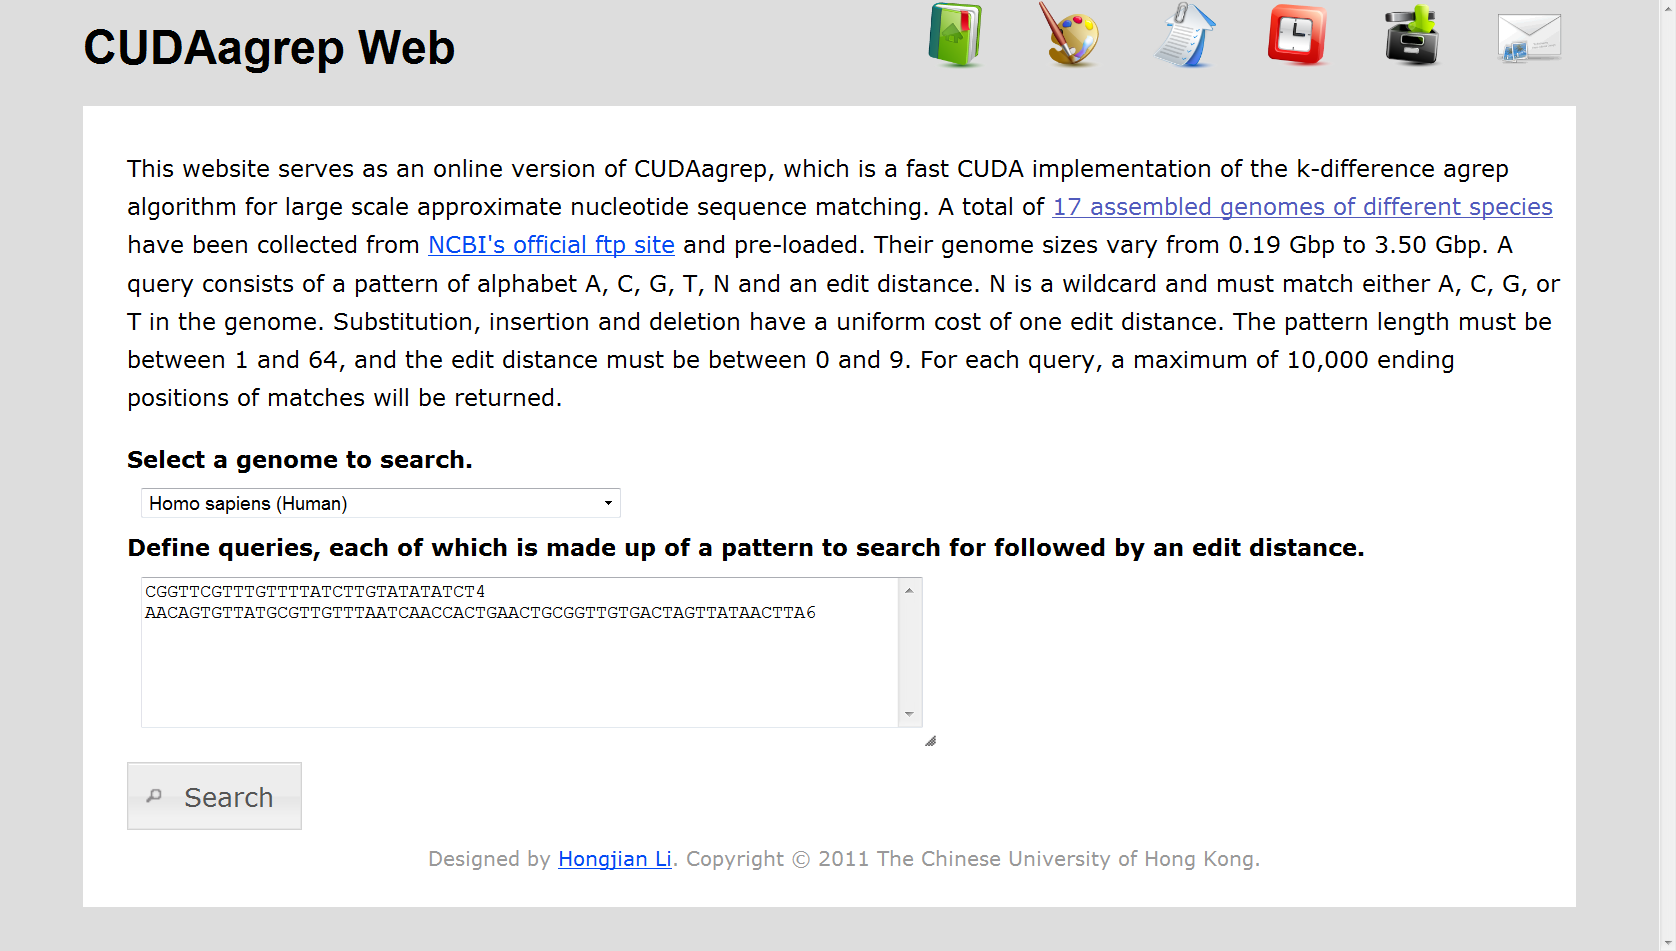
\includegraphics[width=\textwidth]{SequenceMatching/Figures/CUDAagrepWeb.png}
\caption{Snapshot of CUDAagrep website.}
\label{fig:CUDAagrepWeb}
\end{figure}

\begin{figure}
\centering
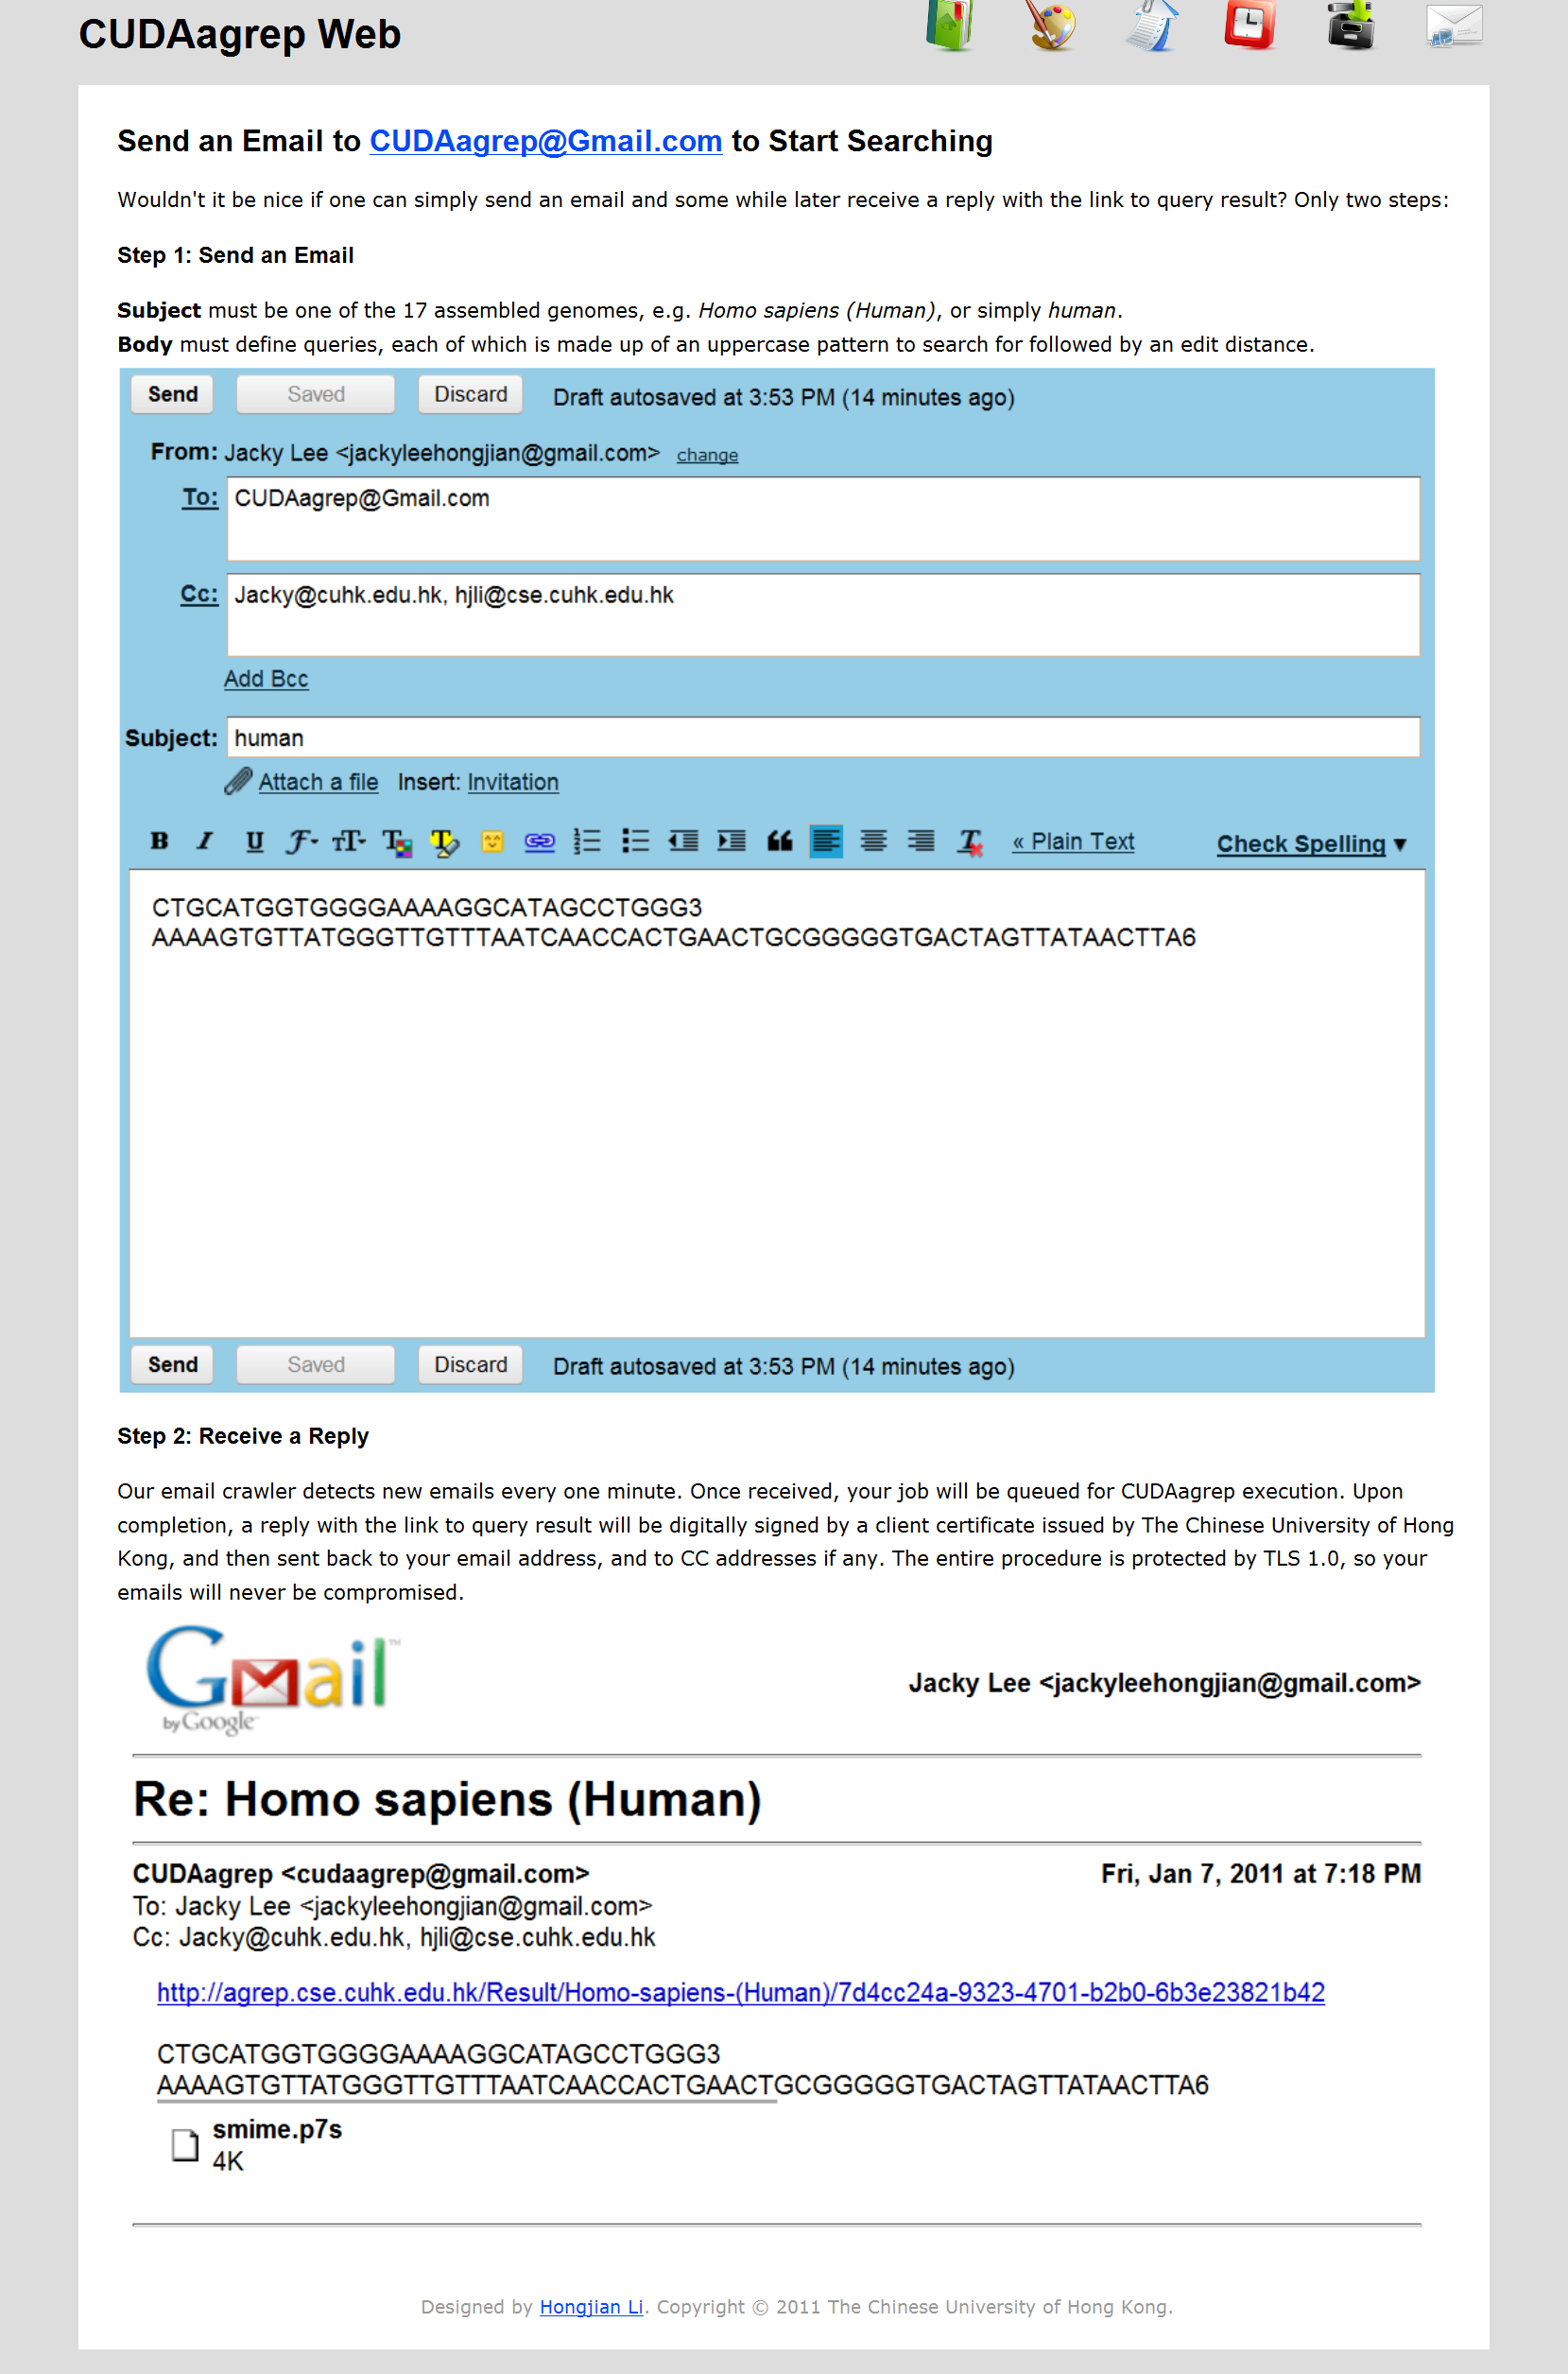
\includegraphics[width=\textwidth]{SequenceMatching/Figures/CUDAagrepEmail.png}
\caption{Snapshot of CUDAagrep email operations.}
\label{fig:CUDAagrepEmail}
\end{figure}

Since the memory requirement of a genome is only one fourth of its original size using binary representation, it is possible for CUDAagrep to load multiple genomes on a desktop computer. In fact, the server hosting our website has already pre-loaded from disk into main memory all the 17 genomes including human, chimpanzee, monkey, rat, mouse, cow, dog, horse, chicken, pig and so on.

\section{Conclusion}

We have developed CUDAagrep, a CUDA implementation of the \textit{K}-difference agrep algorithm for approximate nucleotide sequence matching. The testing results show that it runs very fast, reducing querying time from the magnitude of dozens of seconds down to milliseconds. It requires no indexing at all and thus can be applied in real time. Its high sensitivity is guaranteed by strictly scanning through the entire genome. We have also developed an AJAX MVC website and an email crawler for real time online searching.

\chapterend
